\documentclass[handout,a4paper,slidestop,xcolor=pst,blue]{beamer}

\usepackage{beamerthemesplit}
\usepackage[utf8]{inputenc}
\usepackage[spanish]{babel}
\usepackage{graphicx}
\usepackage{pstricks} % PSTricks package
\usepackage{setspace}
\usepackage{multirow}
\usepackage{listings}
\usepackage{pgfpages}
\usepackage{hyperref}
\usepackage{etoolbox}
\usepackage{epstopdf}

\makeatletter
\patchcmd{\beamer@sectionintoc}{\vskip1.5em}{\vskip0.5em}{}{}
\makeatother

\setbeamercovered{dynamic}
\setcounter{tocdepth}{2}
\setbeamercolor{frametitle}{fg=black,bg=white}
\setbeamercolor{section in toc shaded}{fg=black}
\setbeamercolor{section in toc}{fg=red}
\setbeamercolor{subsection in toc shaded}{fg=black}
\setbeamercolor{subsection in toc}{fg=red}
\setbeamerfont{section in toc}{size=\small}
\setbeamerfont{subsection in toc}{size=\small}
\setbeamertemplate{section in toc shaded}[default][99]
\setbeamertemplate{subsection in toc shaded}[default][99]

\AtBeginSection[]
{\begin{frame}[c]
  \frametitle{Índice}
	\tableofcontents[currentsection,
        sectionstyle=show/shaded,
        subsectionstyle=hide]
\end{frame}}

\AtBeginSubsection[]
{\begin{frame}[c]
	\frametitle{Índice}
	\tableofcontents[
  		currentsection,
  		sectionstyle=shaded/shaded,
  		currentsubsection,
  		subsectionstyle=show/shaded/hide
		]
\end{frame}}

\setbeamercolor{frametitle}{fg=black,bg=white}

\setbeamertemplate{frametitle}{
	\begin{centering}
		\insertframetitle
		\par
	\end{centering}
}

\usetheme[secheader]{Boadilla} 
\usepackage{listings}

\definecolor{pblue}{rgb}{0.13,0.13,1}
\definecolor{pgreen}{rgb}{0,0.5,0}
\definecolor{pred}{rgb}{0.9,0,0}
\definecolor{pgrey}{rgb}{0.46,0.45,0.48}

\lstset{language=Java,
  showspaces=false,
  showtabs=false,
  breaklines=true,
  showstringspaces=false,
  breakatwhitespace=true,
  commentstyle=\color{pgreen},
  keywordstyle=\color{pblue},
  stringstyle=\color{pred},
  basicstyle=\ttfamily,
  keywordsprefix={@}
}


\newcommand{\ann}[1]{\color{blue}\texttt{#1}\color{black}}

\title[JPA + Spring Data]{Capa de Persistencia \\ \ \\ Java Persistence API (JPA) + Spring Data}

\author[P. S{\'a}nchez]{\alert{Pablo S{\'a}nchez}}

\institute[IIE]{
		   Dpto. Ingenier{\'i}a Inform{\'a}tica y Electr{\'o}nica \\
		   Universidad de Cantabria \\
		   Santander (Cantabria, Espa{\~n}a) \\
		   \texttt{p.sanchez@unican.es}
}

\date{}

\begin{document}

\begin{frame}[c]
	\titlepage
	\begin{columns}
		\column{0.50\linewidth}
			\centering
    		
\includegraphics[width=.28\textwidth,keepaspectratio=true]{images/istr.eps}
		\column{0.50\linewidth}
			\centering
			
\includegraphics[width=.25\textwidth,keepaspectratio=true]{images/uc.eps}
	\end{columns}
\end{frame}

\begin{frame}[c]
    \frametitle{\alert{Advertencia}}
    \begin{center}
        Todo el material contenido en este documento no constituye en modo alguno una obra de referencia o apuntes oficiales mediante el cual se puedan preparar las pruebas evaluables necesarias para superar la asignatura. \ \\
        \ \\
        Este documento contiene exclusivamente una serie de diapositivas cuyo objetivo es servir de complemento visual a las actividades realizadas en el aula para la transmisi{\'o}n del contenido sobre el cual versar{\'a}n las mencionadas pruebas evaluables.  \ \\
        \ \\
        Dicho de forma m{\'a}s clara, \alert{estas transparencias no son apuntes y su objetivo no es servir para que el alumno pueda preparar la asignatura.}
    \end{center}
\end{frame}

\section{Introducción}

\begin{frame}
    \frametitle{Puentes de Persistencia de Objetos}
    \rput[lt](0,0){
        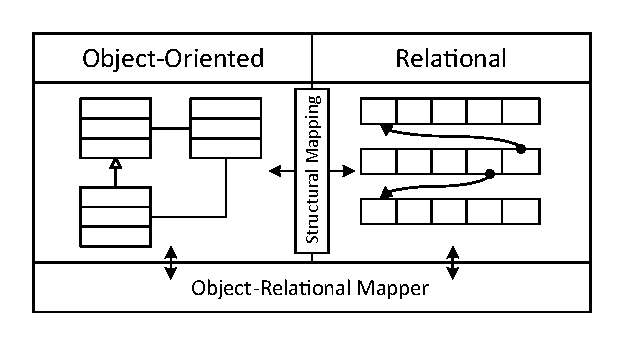
\includegraphics[width=\linewidth]{images/intro/orm02.eps}
    }
\end{frame}

\begin{frame}[c]
    \frametitle{JPA + Spring Data}
    \begin{block}{JPA}
        \emph{Java Persistence API (JPA)} es una especificación de referencia de un puente de persistencia estándar en Java.
        \begin{enumerate}
            \item<2-> Proporciona mecanismos para especificar el \emph{metadata mapping}.
            \item<3-> Especifica la interfaz y funcionamiento que deben tener una serie de elementos para realizar el acceso a datos (e.g. \emph{EntityManager}).
            \item<4-> Precisa de un ORM que la implemente (e.g. Hibernate).
        \end{enumerate}
    \end{block}
    \uncover<5->{
        \begin{block}{Spring Data}
            Framework que proporciona facilidades para la definición de repositorios compatible con diversas tecnologías de persistencia, entre ellas JPA.
        \end{block}
    }
\end{frame}

\begin{frame}[c]
    \frametitle{Objetivos del Tema}
    \begin{enumerate}[<+->]
         \item Ser capaz de transformar un conjunto de POJOs en un esquema relacional usando anotaciones JPA.
         \item Ser capaz crear repositorios JPA y \emph{Spring}.
         \item Ser capaz de utilizar repositorios Spring para interactuar con la capa de persistencia.
    \end{enumerate}
\end{frame}

\begin{frame}[c]
    \frametitle{Bibliografía}
    \begin{thebibliography}{1}

        \bibitem[Bauer, 2015]{Bauer2015}
        Bauer, C., King. G. y Gregory G. (2015).
        \newblock {\em {Java Persistence with Hibernate}}. 2ª Ed.
        \newblock Manning

        \bibitem[Bauer, 2015]{Bauer2015}
        Gierke, O., Darimont, T., Strobl, C., Paluch, M. y Bryant, J. (2019).
        \newblock {\em {Spring Data JPA - Reference Documentation}}.
        \url{https://goo.gl/Fhjdlu}
    \end{thebibliography}
\end{frame}

\section{Transformación Estructural}

\subsection{Metadata Mapping}

\begin{frame}[c]
    \frametitle{Metadata mapping}
    \begin{enumerate}[<+->]
         \item<1-> Se realiza mediante dos alternativas: anotaciones Java o basada en fichero XML.
         \item<2-> Anotaciones Java
             \begin{enumerate}
                \item<3-> Contaminan los POJOs, haciéndolos menos reutilizables y legibles.
                \item<4-> No requieren la actualización de ficheros externos cuando el modelo de dominio evoluciona.
             \end{enumerate}
         \item<5-> Ficheros XML
             \begin{enumerate}
                \item<6-> Permiten tener POJOs más limpios y reutilizables.
                \item<7-> Requieren ser actualizados cuando el modelo de dominio cambia,
             \end{enumerate}
    \end{enumerate}
\end{frame}

\subsection{Entidades y Value Objects}

\begin{frame}[c]
    \frametitle{Entidades y Value Objects}
    \begin{tabular}{lp{0.70\linewidth}}
        \ann{@Entity}     & La clase es una entidad y se transformará a una tabla. \\
        \ann{@Embeddable} & La clase es un \emph{value object} y será incrustada en otra.
    \end{tabular}
\end{frame}

\subsection{Referencias y Colecciones}

\begin{frame}[c]
    \frametitle{Transformación de Propiedades}
    \begin{enumerate}[<+->]
        \item<1-> Basada en campos.
            \begin{itemize}
                \item<2-> Se anotan los atributos a transformar.
                \item<3-> La carga y el almacenamiento se hace basado en reflexión.
            \end{itemize}
        \item<3-> Basada en \emph{getters}.
            \begin{itemize}
                \item<4-> Se anotan los \emph{getters} de los atributos a transformar.
                \item<5-> La carga y almacenamiento se hace basada en \emph{getters} y \emph{setters}.
                \item<6-> Require de \emph{getters} y \emph{setters} públicos para todos los atributos.
            \end{itemize}
    \end{enumerate}
\end{frame}

\begin{frame}[c]
    \frametitle{Transformación de Asociaciones}
    \begin{tabular}{ll}
        \ann{@OneToOne}   & Una referencia simple pertenece a una asociación 1-1. \\
        \ann{@ManyToOne}  & Una referencia simple pertenece a una asociación 1-n. \\
        \ann{@Embedded}   & Una referencia simple será incrustada. \\
        \ann{@OneToMany}  & Una colección pertenece a una asociación 1-n. \\
        \ann{@ManyToMany} & Una colección pertenece a una asociación 1-1. \\
        \ann{@Element}    &  \\
        \multicolumn{1}{r}{\ann{Collection}} & Un colección es de \emph{value objects}. \\
        \ann{@Lob}        & Una referencia se tratará como un LOB. \\
        \ann{@MapKey}     & Permite controlar mejor la transformación de un mapa. \\
    \end{tabular}
\end{frame}

\begin{frame}[c]
    \frametitle{Transformación de Asociaciones - Detalles}
    \begin{tabular}{lp{0.70\linewidth}}
        \ann{cascade}  & Define qué operaciones deben propagarse a la clase referenciada. \\
        \ann{mappedBy} & En una asociación bidireccional, especifica el extremo que hará de clave externo. \\
        \ann{fetch}    & Indica si la referencia se carga bajo demanda (\ann{LAZY}) o no (\ann{EAGER}). \\
    \end{tabular}
\end{frame}

\subsection{Identity Field}

\begin{frame}[c]
    \frametitle{Identity Field}
    \begin{tabular}{lp{0.70\linewidth}}
        \ann{@Id} & El atributo marcado será la clave primaria. \\
        \ann{@GeneratedValue} & El atributo será una clave autogenerada. \\
        \multicolumn{1}{l}{\ann{(strategy=...)}} & Especifica la estrategia de generación. \\
        \multicolumn{1}{r}{\texttt{AUTO}}     & Se deja a decisión del ORM la elección. \\
        \multicolumn{1}{r}{\texttt{IDENTITY}} & Generada por el gestor de pesistencia. \\
        \multicolumn{1}{r}{\texttt{SEQUENCE}} & Usa una \emph{secuencia} del gestor de persistencia. \\
        \multicolumn{1}{r}{\texttt{TABLE}}    & Generada por el propio ORM. \\
        \ann{@IdClass}    & \\
        \ann{@EmbeededId} & Permiten crear claves primarias compuestas.\\
    \end{tabular}
\end{frame}

\subsection{Herencia}

\begin{frame}[c]
    \frametitle{Transformación de Herencias}
    \begin{tabular}{lp{0.70\linewidth}}
        \ann{@Inheritance}                       &  Una clase es raíz de un árbol de herencia.          \\
        \multicolumn{1}{l}{\ann{(strategy=...)}} & Especifica cómo se transforma un árbol de herencia.  \\
        \multicolumn{1}{r}{\texttt{SINGLE\_TABLE}}    & Aplica \emph{Single Table Inheritance}    \\
        \multicolumn{1}{r}{\texttt{JOINED}}          & Aplica \emph{Class Table Inheritance}     \\
        \multicolumn{1}{r}{\texttt{TABLE\_PER\_CLASS}} & Aplica \emph{Concrete Table Inheritance}  \\
    \end{tabular}
\end{frame}

\subsection{Personalización y Optimización}

\begin{frame}[c]
    \frametitle{Opciones de Personalización y Optimización}
    \begin{tabular}{lp{0.70\linewidth}}
        \ann{@Table}      & Personaliza las tablas ligadas a una \ann{@Entity}. \\
        \ann{@Column}     & Personaliza las columnas ligadas a un atributo. \\
        \ann{@JoinColumn} & Personaliza las claves fóraneas en \emph{Foreign Key} \\
        \ann{@JoinTable } & Personaliza las tabla intermedia en \emph{Association Table}. \\
        \ann{@Unique}     & \\
        \multicolumn{1}{r}{\ann{Constraint}} & Especifica restricciones de unicidad adicionales. \\
        \ann{@Discriminator} &  \\
        \multicolumn{1}{r}{\ann{Column}} & Personaliza la columna \emph{tipo} en \emph{Single Table}. \\
        \ann{@Discriminator} &  \\
        \multicolumn{1}{r}{\ann{Value}} & Personaliza los valores de \emph{tipo} en \emph{Single Table}. \\
    \end{tabular}
\end{frame}

\section{Spring Repositories}

\subsection{Introducción}

\begin{frame}[c]
    \frametitle{Spring Repositories}
    \begin{enumerate}[<+->]
        \item Facilidad que permite la generación automática de repositorios a partir de la extensión de una interfaz de alto nivel.
        \item Soporte implícito para las operaciones básicas comunes.
        \item Soporte avanzado para operaciones más específicas.
        \item Facilidades de personalización avanzada.
        \item Soporte para paginación, ordenado, \emph{streams} y métodos asíncronos.
        \item Soporte para \emph{query by example}.
        \item Soporte para \emph{data transfer objects}.
    \end{enumerate}
\end{frame}

\begin{frame}[c]
    \frametitle{Jerarquía de los Spring Repositories}
    \begin{center}
        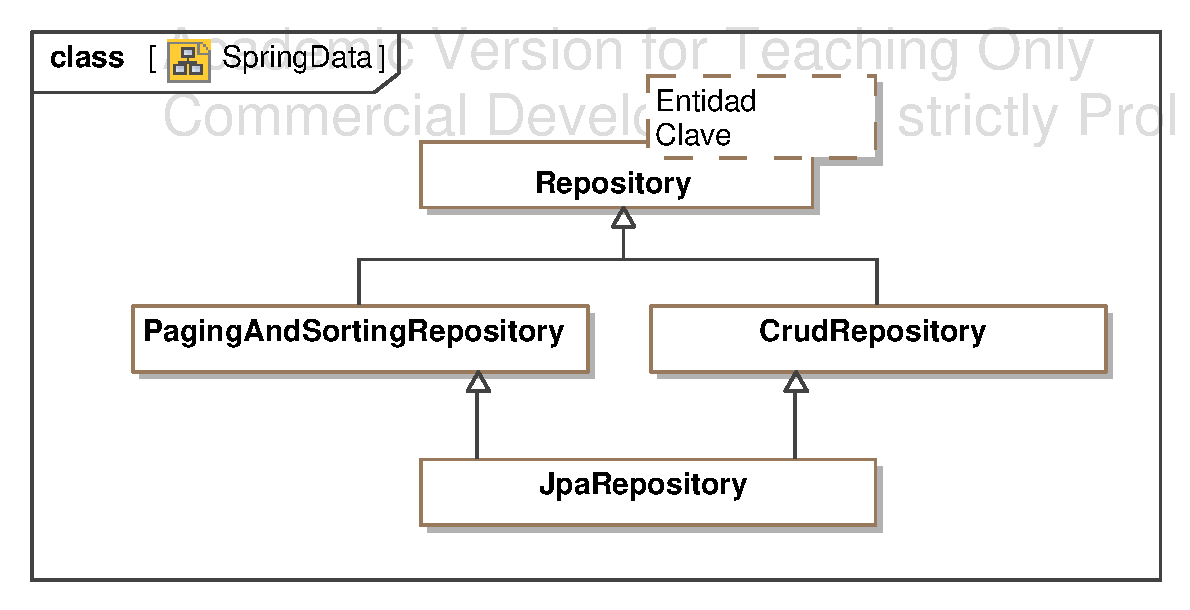
\includegraphics[width=.8\linewidth]{images/spring/SpringData.eps}
    \end{center}
\end{frame}

\subsection{Interfaces de los Repositorios}

\begin{frame}[c,fragile]
    \frametitle{Repositorios CRUD}
    \begin{lstlisting}[basicstyle=\footnotesize,language=Java]
public interface CrudRepository<T, ID extends Serializable>
  extends Repository<T, ID> {

  <S extends T> S save(S entity);

  Optional<T> findById(ID primaryKey);

  Iterable<T> findAll();

  long count();

  void delete(T entity);

  boolean existsById(ID primaryKey);}

\end{lstlisting}
\end{frame}

\begin{frame}[c,fragile]
    \frametitle{Repositorios Page and Sorting}
    \begin{lstlisting}[basicstyle=\footnotesize,language=Java]
public interface PagingAndSortingRepository<T, ID extends Serializable>
  extends CrudRepository<T, ID> {

    Iterable<T> findAll(Sort sort);

    Page<T> findAll(Pageable pageable);
}
    \end{lstlisting}
\end{frame}

\begin{frame}[c,fragile]
    \frametitle{Repositorios JPA}
    \begin{lstlisting}[basicstyle=\footnotesize,language=Java]
public interface JpaRepository<T, ID extends Serializable> extends
  PagingAndSortingRepository<T, ID> {

    List<T> findAll();

    List<T> findAll(Sort sort);

    List<T> save(Iterable<? extends T> entities);

    void flush();

    T saveAndFlush(T entity);

    void deleteInBatch(Iterable<T> entities);
}
    \end{lstlisting}
\end{frame}

\begin{frame}[c,fragile]
    \frametitle{Crear un Spring Repository}
\begin{lstlisting}[basicstyle=\small,language=Java]
public interface ViajeRepository extends JpaRepository<Viaje,Long>{}
\end{lstlisting}
\end{frame}

\begin{frame}[c,fragile]
    \frametitle{Inyectar un Spring Repository JPA}
\begin{lstlisting}[basicstyle=\footnotesize,language=Java]
public class ViajeService {
	
  @Autowired
  protected ViajeRepository vr;	

  public boolean cerrarViaje(Long id) throws ViajeNotFound {
		
    Viaje v = vr.findById(id).orElseThrow(ViajeNotFound::new);
		
  }
}
\end{lstlisting}
\end{frame}

\subsection{Consultas Avanzadas}

\begin{frame}[c]
    \frametitle{Creación de Operaciones Personalizadas}
    \begin{enumerate}[<+->]
        \item Definidas a través de los nombres de los métodos.
        \item Definidas a través de expresiones JPQL (Java Persistence Query Language).
        \item Definidas a través de \emph{especificaciones}.
        \item Definidas a través de \emph{Query By Example}.
    \end{enumerate}
\end{frame}

\begin{frame}[c,fragile]
    \frametitle{Personalización mediante Nombres de Métodos}
\begin{lstlisting}[basicstyle=\footnotesize,language=Java]
public interface UsuarioRepository extends JpaRepository<Usuario,String> {
	
	Usuario findByEmail(String email);
	
	Set<Usuario> findByFechaAltaAfter(Date fecha);

}
\end{lstlisting}
\end{frame}

\begin{frame}[c,fragile]
    \frametitle{Personalización mediante Nombres de Métodos}
    \begin{center}
    \begin{tabular}{l|l}
    Keyword              & Ejemplo                                     \\ \hline
    \ann{findBy,countBy} & \texttt{findByEmail}, \texttt{findByEmail}  \\
    Navegación           & \texttt{findByOrigenCiudad}                 \\
    \ann{And, Or}        & \texttt{findByOrigenCiudadAndDestinoCiudad} \\
    \ann{Like}           & \texttt{findByOrigenCiudadLike}             \\
    \ann{IgnoreCase}     & \texttt{findByOrigenCiudadLikeIgnoreCase}   \\
    \ann{Between}        & \texttt{findByFechaBetween}           \\
    \ann{LessThan}       & \texttt{findByPrecioLessThan}         \\
    \ann{After, Before}  & \texttt{findByFechaBefore}            \\
    \ann{Not}            & \texttt{findByConductorNombreNot}     \\
    \ann{OrderBy(Desc)}  & \texttt{findByPriceOrderByPriceAsc}   \\
    \end{tabular}
    \end{center}
\end{frame}

\begin{frame}[c,fragile]
    \frametitle{Personalización mediante Nombres de Métodos}
\begin{lstlisting}[basicstyle=\footnotesize,language=Java]
public interface ViajeRepository
                   extends JpaRepository<Viaje,Long>
{
  public Set<Viaje>
     findByOrigenCiudadAndDestinoCiudad(
          String ciudadOrigen,
          String ciudadDestino);
	
  public Set<Viaje>
     findByOrigenCiudadAndFechaBeforeOrderByPrecio(
          String ciudad,
          Date fecha);
}
\end{lstlisting}
\end{frame}


\begin{frame}[c,fragile]
    \frametitle{Personalización mediante JPQL}
\begin{lstlisting}[basicstyle=\footnotesize,language=Java]
public interface ViajeRepository
                   extends JpaRepository<Viaje,Long> {
	
	@Query("SELECT v FROM Viaje v
                    WHERE v.origen.ciudad = ?1
                      AND v.destino.ciudad = ?2")
	public Set<Viaje> findByOrigenAndDestino(
                                      String origen,
                                      String destino);
}
\end{lstlisting}
\end{frame}

\section{Sumario}

\begin{frame}[c]
    \frametitle{¿Qué tengo que saber de todo ésto?}
    \begin{enumerate}[<+->]
        \item Ser capaz de utilizar anotaciones JPA para especificar una correspondencia objeto-relacional.
        \item Ser capaz de definir repositorios \emph{JPA} en \emph{Spring}.
        \item Ser capaz de utilizar repositorios \emph{JPA} en \emph{Spring}.
    \end{enumerate}
\end{frame}

\end{document}
